% ---
% Ambiente de desenvolvimento com Sublime Text
% ---
\chapter{Ambiente de desenvolvimento com Sublime Text}
\label{cap2}
% ---

Ao final deste capítulo, o aluno terá as seguintes competências:
\begin{enumerate}
	\item Instalar o \sublime~\sublimeversao~no sistema operacional;
	\item Instalar \plugins~do \sublime; e
	\item Criar uma estrutura de aplicação \web~com \php. 
\end{enumerate}

\section{O \sublime}
\label{o-sublime}

O \sublime~é um editor de textos melhorado. Com esse tipo de \software~
é possível desenvolver os mais diversos programas, incluindo os \sites. 
O \sublime~hoje dispõe de duas versões que são amplamente utilizadas. 
A versão 2 - estável porém mais antiga e a versão \sublimeversao~- caracterizada como 
versão \textit{beta} porém mais nova. Apesar de no curso sempre trabalharmos com 
as versões estáveis dos programas, com esse editor usaremos a versão \sublimeversao.

O editor de textos não vem por padrão nas distribuições Linux. Por isso, é necessário instalá-lo. 
Vamos abrir o navegador Firefox e digitar a URL \url{https://www.sublimetext.com/3}.
Em seguida, clique no \textit{link} ``Download''. Se você estiver usando o Linux do Projeto e-Jovem
escolha a opção ``Ubuntu 32 bit''. Essa ação vai baixar o arquivo \sublimefilename.
o \texttt{3XXX} indica a versão (\sublimeversao~no caso) e pequenas mudanças na 
versão principal respectivamente.

Lembre-se! Saíba onde você salvou o arquivo baixado! Será importante saber a 
localização dele no momento da instalação!

\section{Instalando o \sublime}
\label{instalando-o-sublime}

Agora que baixamos o arquivo \texttt{.deb}, vamos instalá-lo. Abra o \terminal~de acordo
com o apresentado na seção \ref{instalacao-do-php}. Utilize os comandos \comandocdcompleto, 
\comandolscompleto~e \comandopwdcompleto~para ir ao diretório que o arquivo 
\sublimefilename~está salvo. No caso da apostila, o arquivo foi salvo dentro do 
diretório \directory{/home/ejovem/Downloads}.

Caso você não saíba onde o arquivo se encontra, peça ajuda ao seu instrutor.

\begin{multicols}{2}

  Comandos executados no terminal 
  \begin{lstlisting}[language=bash,style=codigos]
    $ cd ~/Downloads
    $ ls
  \end{lstlisting}

  \columnbreak

  Resposta do comando \comandolscompleto
  \begin{lstlisting}[language=bash, style=codigos]
    ...  
    sublime-text_build-3114_i368.deb
    ...  
  \end{lstlisting}

\end{multicols}

Agora que a gente sabe onde o arquivo se encontra, podemos instalar com o comando
\dpkg. Execute o seguinte código no diretório em que o \sublimefilename~se encontra

  \begin{lstlisting}[language=bash,style=codigos]
    $ sudo dpkg -i sublime-text_build-3114_i368.deb
  \end{lstlisting}

Se a instalação do \sublime~ocorreu com sucesso. Obtemos a seguinte tela na 
imagem \ref{fig:sublime-instalacao-ok}. Para abrir o programa, digite a combinação 
de teclas \altfdois~e digite o comando \sublimebin. A tela inicial do programa é 
a exibida na figura \ref{fig:sublime-ok}.

\figuradupla{sublime-instalacao-ok}{Instalação do aplicativo \sublime~realizada com sucesso}
{sublime-ok}{Tela inicial do \sublime}

\section{Primeiros passos}
\label{primeiros-passos}

Vamos começar nossos testes com o \sublime. Nosso primeiro teste é abrir o arquivo 
editado anteriormente pelo programa \gedit. Na tela inicial do \sublime, execute a seguinte
sequência de menus: \menu[,]{File, Open File...}. O arquivo deverá estar no diretório
\directory{/var/www/aula01}. E tem o nome de \arquivo{index.php}.

Vamos editar o arquivo. Troque a primeira linha do arquivo para que fique parecido com o
apresentado abaixo.

\lstinputlisting[language=php,style=codigos]{codigos/echo-sublime.php}

Lembre-se! Você pode colocar \tags~\html~dentro das instruções \php!

O resultado pode ser conferido abaixo.

\figurasimples{sublime-echo-ok}{Utilizando \funcaoecho.}

\section{Comandos do \sublime}
\label{comandos-do-sublime}

O nosso editor de textos tem um painel de comandos. Nele é possível aplicar comandos
relacionados ao \sublime. Os comandos que iremos utilizar são em inglês, portanto,
a tabela TAL trás a tradução de alguns termos utilizados.

Para acessar o painel digite a combinação de teclas \ctrlshiftp~enquanto estiver
no \sublime. O painel deve aparecer na parte superior da janela. Digite o termo
\sidebar. Esse termo ativará o comando de nome \textit{View: Toggle Side Bar}.
Esse comando ativa ou desativa a barra lateral no \sublime~(pode ser utilizado
a combinação de teclas \sublimesidebar). 

Outro comando que podemos utilizar é o de ativar ou desativar o \textit{minimap}. 
Pressione então as teclas \ctrlshiftp~e digite o termo \textit{minimap}. 
O comando completo é \textit{View: Toggle Minimap}.

\section{Adicionando diretórios}
\label{adicionando-diretorios}

Uma das grandes facilidades do editor de textos \sublime~e outros editores mais
avançados é a apresentação do projeto através da barra lateral (\textit{sidebar}).
No nosso caso, um projeto pode ser descrito simplesmente como uma pasta. Então
vamos adicionar a pasta \directory{aula01} ao \sublime. 

Para isso, abra o programa gerenciador de arquivos do sistema. No caso da 
distribuição do e-Jovem, o programa a ser aberto é o \thunar. Pressione a 
combinação de teclas \altfdois~em seguida digite \thunar. Navegue até o 
diretório \directory{/var/www/} clique em cima da pasta \directory{aula01} 
segure e arraste até o editor de textos \sublime.

\begin{figure}[H]
  \begin{center}
    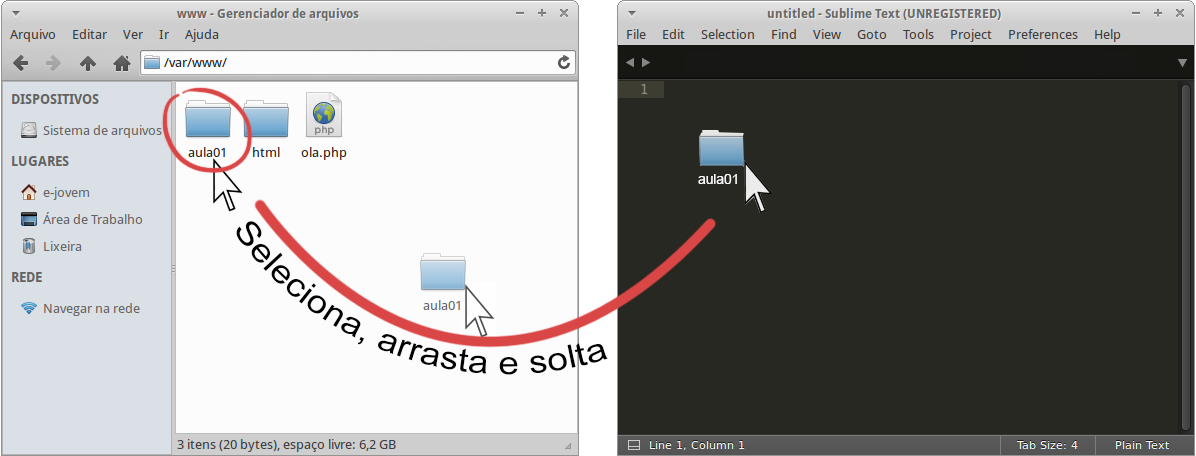
\includegraphics[width=14cm]{adicionando-diretorios}
    \caption{Adicione diretório ao \sublime~de maneira
simples, clique em uma pasta e arraste para dentro do editor.}
    \label{fig:adicionando-diretorios}
  \end{center}
\end{figure}

Nesse momento a tela principal do \sublime~encontra-se com a \sideb~(barra lateral)
ativada e apresentando o diretório que acabamos de adicionar.

\figurasimples{sublime-projeto-ok}{Programa \sublime~com barra lateral visível.}

Dica! Outro método que podemos utilizar para realizar a mesma tarefa é utilizar
os menus do \sublime. O caminho a ser percorrido é: \menu[,]{File, Open Folder...}
e escolher o diretório \directory{/var/www/aula01}.


\section{Configurações do Usuário}
\label{configuracoes-do-usuario}

O \sublime~permite diversas modificações no seu funcionamento a partir das configurações
que o usuário (no caso você) pode realizar. Você deve editar o arquivo 
que se encontra no menu \menu[,]{Preferences, Settings - User}.

Edite o arquivo para que fique parecido com o código abaixo. Você pode procurar
na internet por mais comandos que modifiquem o comportamento do \sublime.

\lstinputlisting[style=codigos]{codigos/settings-user.json}

\section{Configurações e Plugins}
\label{configuracoes-e-plugins}

O \sublime~se tornou famoso por conta da possibilidade de adicionarmos à ele,
diversas outras funcionalidades por meio de \plugins. Existem \plugins~que auxiliam
no desenvolvimento de \html, \css~e em diversas outras linguagens.

Para tirar o maior proveito dos \plugins, vamos adicionar um gerenciador de
\plugins~ao nosso \sublime.

Vamos acessar o site \url{http://packagecontrol.io/installation} através do navegador 
Firefox. Copie toda o código representado na figura \ref{fig:sublime-packagecontrol-installation}.

Agora devemos ir até o \sublime~e seguir o caminho \menu[,]{View, Show console...}.
Uma pequena seção irá aparecer na parte debaixo da tela principal do programa.
Usando o botão direito do \mouse, clique no campo como mostrado na figura 
\ref{fig:sublime-packagecontrol-paste-code} escolha a opção \textit{paste} (colar em inglês)
e pressione \avancar. Após a finalização da instalação, percorra o menu \menu[,]{View, Hide console...} 
para esconder o \terminal.

\figuradupla{sublime-packagecontrol-installation-2}{Código que deve ser copiado, 
em seguida, colado no \sublime.}{sublime-packagecontrol-paste-code}{Opção a ser
escolhida para colar código copiado anteriormente}

\subsection{Plugin \texttt{php-snippets}}
\label{plugin-php-snippets}

Como teste, instalaremos o pacote \texttt{php-snippets}. Esse
pacote nada mais é do que um conjunto de códigos pré-prontos. Inicialmente não
nos terá muita serventia, mas com o passar das aulas será bem útil.

Para instalar um \plugin~precisamos executar alguns comandos no painel de comandos.
Com o \sublime~aberto, digite a combinação de teclas \ctrlshiftp~e digite
\textit{package install}. Esse termo ativará o comando \textit{Package Control: Install Package}.
Ao pressionar \avancar~o painel de comandos listará todos os pacotes disponíveis
para instalação. Digite o termo \textit{php-snippets}, ativando assim, o pacote
de nome \textit{php-snippets}. Veja a figura

\figurasimples{sublime-plugin-installation}{Instalação do \plugin~\texttt{php-snippets}.} 

\section{Desafio!}
\label{cap2-desafio}
O desafio deste capítulo é você configurar o \sublime~de acordo com o seu gosto.
Modifique os seguintes itens:
\begin{enumerate}
  \item Tamanho e tipo da fonte.
  \item Cor do editor (\menu[,]{Preferences, Color Scheme, <opção>})
  \item Instalar o \plugin~\texttt{phpdoc}~ (\url{https://packagecontrol.io/packages/PhpDoc}).
\end{enumerate}
